\documentclass[10pt,twocolumn,letterpaper]{article}

\usepackage{cvpr}
\usepackage{times}
\usepackage{epsfig}
\usepackage{graphicx}
\usepackage{amsmath}
\usepackage{amssymb}
\usepackage{tikz}
\usepackage{tikz-qtree}

% Include other packages here, before hyperref.

% If you comment hyperref and then uncomment it, you should delete
% egpaper.aux before re-running latex.  (Or just hit 'q' on the first latex
% run, let it finish, and you should be clear).
\usepackage[breaklinks=true,bookmarks=false]{hyperref}

\cvprfinalcopy % *** Uncomment this line for the final submission

\def\cvprPaperID{****} % *** Enter the CVPR Paper ID here
\def\httilde{\mbox{\tt\raisebox{-.5ex}{\symbol{126}}}}

% Pages are numbered in submission mode, and unnumbered in camera-ready
%\ifcvprfinal\pagestyle{empty}\fi
% \setcounter{page}{4321}
\begin{document}

%%%%%%%%% TITLE
\title{A Survey of NeRF for Sparse Views}

\author{Yuxuan Kuang\\
School of EECS, Peking University\\
% Institution1 address\\
{\tt\small kuangyuxuan@stu.pku.edu.cn}
% For a paper whose authors are all at the same institution,
% omit the following lines up until the closing ``}''.
% Additional authors and addresses can be added with ``\and'',
% just like the second author.
% To save space, use either the email address or home page, not both
% \and
% Second Author\\
% Institution2\\
% First line of institution2 address\\
% {\tt\small secondauthor@i2.org}
}

\maketitle
%\thispagestyle{empty}

%%%%%%%%% ABSTRACT
% \begin{abstract}
%    In this paper, I systematically survey the NeRF model for sparse views.
%    I first analyze the shortcomings and difficulties of the original NeRF model,
%    then I introduce the variants of NeRF for sparse views, analyze their inner relations and compare their abilities.
%    Finally, I point out my personal opinions on the future development of NeRF for sparse views.
% \end{abstract}

%%%%%%%%% BODY TEXT
% introduction
% related works (contributions)
% Relationship between variants
% my opinions and future plans

\section{Introduction}

Neural radiance fields (NeRF)~\cite{mildenhall2020nerf} encode a scene into a neural representation that enables photo-realistic rendering of novel views. However, a successful reconstruction from RGB images requires a large number of input views taken under static conditions — typically up to a few hundred images for room-size scenes.
Moreover, the speed of NeRF is disastrously slow because of the hundreds of views it needs to process.
As a result, how to use NeRF for 3D reconstruction leveraging very few images is quite important.
In this survey, I will introduce the variants of NeRF which are able to leverage sparse views — even single view to reconstruct 3D scenes.

\section{Related Works}

To tackle this tricky problem, many methods have been proposed.
In Figure \ref{fig:taxonomy}, selected methods are grouped into different perspectives that these methods are based on.
For each perspective, a few works will be mentioned and their contributions will be explained.

\begin{figure}[h]
   \begin{center}
      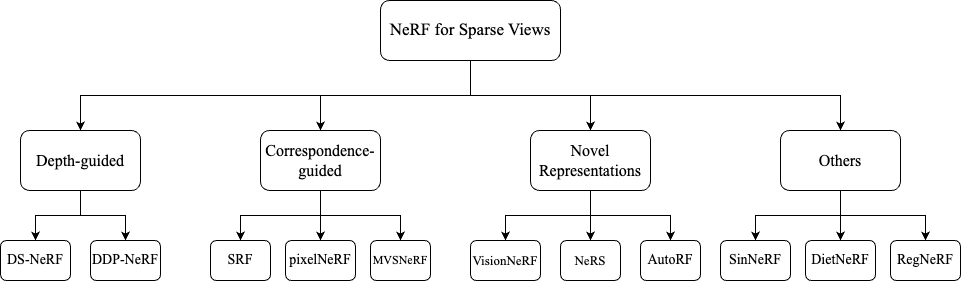
\includegraphics[width=80mm]{assets/taxonomy.png}
   \end{center}
   \caption{Taxonomy of NeRF for Sparse Views}
   \label{fig:taxonomy}
\end{figure}

\subsection{Using Depth to Guide Reconstruction}

It is very common to use depth information to guide 3D reconstruction, since in multi-view stereo, coarse 3D information can be easily obtained by Structure from Motion (SfM).

In DS-NeRF~\cite{kangle2021dsnerf}, researchers use SfM to produce sparse 3D points that can be used as “free” depth supervision during training
and add a loss to encourage the distribution of a ray’s terminating depth matches a given 3D keypoint, incorporating depth uncertainty.

While in DDP-NeRF~\cite{Roessle_2022_CVPR}, researchers first utilize the sparse point cloud reconstructions from SfM preprocessing, which to feed into a depth completion network. They then impose these depth estimates as constraints to the NeRF optimization according to the estimated uncertainty.

Both of the two works facilitate novel view synthesis results at significantly higher image quality and lower depth error compared to NeRF, and more importantly, they both use depth information to help constraint NeRF and achieve sparse-view reconstruction.

\subsection{Leveraging Correspondences between 2D and 3D}

Since we know NeRF is the neural bridge between 2D and 3D, then it is natural to use the correspondences between 2D and 3D to help the reconstruction.

In SRF~\cite{SRF}, researchers predict color and density for each 3D point given an encoding of its stereo correspondence in the input images. The encoding is implicitly learned by an ensemble of pair-wise similarities — emulating classical stereo. Experiments show that SRF learns structure instead of over-fitting on a scene.

In~\cite{yu2020pixelnerf}, researchers proposed pixelNeRF, a learning framework that enables predicting NeRFs from one or several images in a feed-forward manner. Unlike the original NeRF network, which does not make use of any image features, pixelNeRF takes spatial image features aligned to each pixel as an input. This image conditioning allows the framework to be trained on a set of multi-view images, where it can learn scene priors to perform view synthesis from one or few input views.

And in MVSNeRF~\cite{mvsnerf}, researchers leverages plane-swept cost volumes (widely used in multi-view stereo) for geometry-aware scene reasoning, and combines this with physically based volume rendering for neural radiance field reconstruction.
They first constructs a cost volume by warping 2D image features onto a plane sweep, then apply 3D CNN to reconstruct a neural encoding volume with per-voxel neural features, which they use to interpolate features to regress volume density and RGB radiance by an MLP.

\subsection{Applying Novel Representations}

NeRF~\cite{mildenhall2020nerf} proposed a neural representation of 3D scenes, but it also has a few drawbacks, like lacking the ability to capture the global structure of the scene. A few works addressed these drawbacks by applying novel representations which are inspired by the original architecture of NeRF.

In VisionNeRF~\cite{lin2023visionnerf}, researchers from UC San Diego and MIT propose to leverage both the global and local features to form an expressive 3D representation. The global features are learned from a vision transformer, while the local features are extracted from a 2D convolutional network. 
Therefore, this novel 3D representation allows the network to reconstruct unseen regions without enforcing constraints like symmetry or canonical coordinate systems.

While NeRS~\cite{zhang2021ners} learns a neural shape representation of a closed surface that is diffeomorphic to a sphere, guaranteeing water-tight reconstructions. Even more importantly, surface parameterizations allow NeRS to learn (neural) bidirectional surface reflectance functions (BRDFs) that factorize view-dependent appearance into environmental illumination, diffuse color (albedo), and specular “shininess.”

And in \cite{mueller2022autorf}, AutoRF is proposed to learn a normalized, object-centric representation whose embedding describes and disentangles shape, appearance, and pose. Each encoding provides well-generalizable, compact information about the object of interest, which is decoded in a single-shot into a new target view, thus enabling novel view synthesis.

\subsection{Others}

Of course, apart from the above perspectives, there are methods that make use of other elaborated ideas to achieve sparse-view reconstruction.

The core idea of learning scene representation from sparse input is the idea of semi-supervised learning, where psuedo labels play an important role. 
In \cite{Xu_2022_SinNeRF}, researchers present a Single View NeRF (SinNeRF) framework consisting of thoughtfully designed semantic and geometry regularizations.
Specifically, SinNeRF constructs a semi-supervised learning process, where geometry pseudo labels and semantic pseudo labels are introduced to guide the progressive training process.

Using semantic consistency is also a novel perspective to look at. In DietNeRF~\cite{Jain_2021_ICCV}, an auxiliary semantic consistency loss is introduced to encourage realistic renderings at novel poses and allow it to get supervision from arbitrary poses. They leverage CLIP~\cite{DBLP:journals/corr/abs-2103-00020} vision encoder to get semantic similarities and use the consistency for supervision, thus improving the perceptual quality of few-shot view synthesis when learned from scratch.

Finally, in RegNeRF~\cite{Niemeyer2021Regnerf}, researchers observe that the majority of artifacts in sparse input scenarios are caused by errors in the estimated scene geometry, and by divergent behavior at the start of training. Therefore they address this by regularizing the geometry and appearance of patches rendered from unobserved viewpoints, and annealing the ray sampling space during training. They additionally use a normalizing flow model to regularize the color of unobserved viewpoints.

\section{Relationship between NeRF Variants}

\section{Future Development}

\newpage
{\small
\bibliographystyle{ieee}
\bibliography{egbib}
}

\end{document}
